\documentclass[]{scrartcl}

\newif\ifhtml

% HTML generation (.doc-conversion) > set html to true and use htlatex. else set html to false
\htmltrue
\htmlfalse

\ifhtml % In case of web format output...
	\def\pgfsysdriver{pgfsys-tex4ht.def}
\else
\fi

\usepackage[ansinew]{inputenc}	% so I can write my Name without \"{u}
\usepackage[T1]{fontenc}		% Standard Latex-Fonts
\usepackage[english]{babel}		% change [english] if written in other language
\usepackage{svn-multi}			% to add SVN-Versioning-Info
\usepackage{graphicx}
\usepackage{subfig}				% subfigures
\usepackage[Gray]{SIunits}		% typographically correct units (\milli\meter, \kilo\electronvolt)
\usepackage{booktabs}			% nice tables
\usepackage{fancyhdr}			% nice header
\usepackage{tikz}				% extremely nice drawings
\usepackage{microtype}			% for nicer typography
\usepackage[numbers,square,sort&compress]{natbib} % nice bibliography
\usepackage{caption}
\usepackage{relsize} 			% for nice C++ (from http://tinyurl.com/5hllnf)
%\usepackage{setspace}
%	\doublespacing
%	\onehalfspacing
%	\singlespacing

\ifhtml
	\usepackage{index}
	\usepackage{color}
	\newindex{todo}{todo}{tnd}{Todo List} 
	\newcommand{\todo}[1]{\textcolor{red}{[To do: #1]}\index[todo]{#1}}
	\usepackage{hyperref}
\else
	\usepackage{lmodern}
	%\usepackage{lineno}
	% line numbers
	%\linenumbers
	%%\pagewiselinenumbers
	%\modulolinenumbers[2]
	\usepackage[backref]{hyperref}			% backref generates link from references back to text
	\usepackage{todonotes}
	\hypersetup{%
			pdfauthor={David Haberth�r},%
			pdftitle={Progress Report for the Graduate School for Cellular and Biomedical Sciences - 2008},%
			pdfsubject={Progress Report},%
			pdfkeywords={skeletonization, tomography, biomedical imaging, SRXTM},%
			colorlinks=false % colored links (true or false)
			}
\fi

%% Subversion Information
\svnidlong
{$HeadURL$}
{$LastChangedDate$}
{$LastChangedRevision$}
{$LastChangedBy$}
\svnid{$Id$}

\pagestyle{fancy}
%%%
%\cfoot{}
%\rfoot{}
%%%
%\fancyhead{}
%\fancyfoot{}
%\fancyhead[RO]{{\footnotesize\rightmark}}
%\fancyfoot[RO]{\thepage}
%\fancyhead[LE]{{\footnotesize\leftmark}}
%\fancyfoot[LE]{\thepage}
%%svn-info in footer, page in header
%\fancyfoot[C]{\tiny{this document (\url{\svnkw{HeadURL}}) was last saved on \svnkw{LastChangedDate} by \svnkw{LastChangedBy} and is now on revision \svnkw{LastChangedRevision}.}}
%\fancyhead[C]{page \thepage}

%\pagestyle{headings}
%\pagestyle{plain}

\newcommand{\imsize}{\linewidth}

% define nicely typeset C++
\def\ifmonospace{\ifdim\fontdimen3\font=0pt }
%c C plus plus
	\def\C++{%
	\ifmonospace%
	C++%
	\else%
	C\kern-.1667em\raise.30ex\hbox{\smaller{++}}%
	\fi%
	\spacefactor1000 }
%

\title{Progress Report for the Graduate School for Cellular and Biomedical Sciences - 2008}
\author{David Haberth�r}
\date{January 6, 2009}

\begin{document}

\maketitle

\ifhtml
	\emph{Did you sort out all to dos?}
\else
	%\listoftodos
\fi

%\tableofcontents

\section{Overview}
Corresponding to my last submitted progress report from February 19, 2008, I focused on different tasks during the past year. All my work revolves around the data obtained with synchrotron radiation based x-ray tomographic imaging (SRXTM) at the TOMCAT beamline~\cite{Stampanoni2007} of the Swiss Light Source (SLS) at the Paul Scherrer Institut (PSI) in Villigen, Switzerland.

The past year I have worked on multimodal imaging to detect sub-micron particles in the lung and on the skeletonization of the terminal airways. As I have stated in the last progress report, the multimodal imaging approach I was working on has been superseded by recent progressions at TOMCAT and is for the moment no longer actively followed by our group. Nevertheless we were able to match results from two imaging modalities; the results obtained with this multimodal imaging method, the nanoparticle detection and the assessment of the agreement between conventional electron microscopy and SRXTM are all described in section~\ref{sec:multimodal imaging}.

In addition to this, I have worked on the extraction of the airway structure---the branching pattern of the airways, the lengths and angles of different segments---from tomographic datasets. The three dimensional structure of the gas-exchanging airways influences the airflow patterns in the lung, particle deposition in the terminal airways depends on the lung structure and different mice and rat strains exhibit a different branching pattern during lung development. The structure of the airways and the branching pattern can be described using the so called airway skeleton. I have developed a method to extract structural information from SRXTM data sets, the details of this method are described in section~\ref{sec:skeletonization}.

During the past summer I had the possibility to conduct the thesis of my Master of Advanced Studies ETH in Medical Physics directly involved with the development of a new scanning protocol, working for two full months at the TOMCAT beamline at the PSI, while being integrated in the group we otherwise closely collaborate. The developed method is planned to be implemented for end-user access at the beamline early in 2009. This so called wide field scanning method is described in section~\ref{sec:wide field scanning}.

\section{SRXTM}
During three regularly allotted beam times we obtained tomographic datasets of 67~samples while performing 151~scans in total. The difference between the amount of scanned samples and total scans arises through the use of a novel imaging method, which uses multiple partial scans to obtain tomographic images of one sample and is described later on in section~\ref{sec:wide field scanning}. During the term of my master thesis I additionally performed 17~scans---each with three or five subscans---during the so called ``in house development'' time at the beamline to proof the simulated predictions made during the development of the wide field scanning method.

Most of the samples recorded were obtained from lung samples from Sprague Dawley rats (see~\cite{Schittny2008} for details on the animals and sample preparation). During the third beamtime in 2008 we also obtained tomographic scans of mice bones (tibia, femur and vertebrae) to asses the trabecular structure of these bones. This particular experiment has been performed as part of a collaboration with the University of G�ttingen, Germany, which has an ongoing program where skeletal morphology of rodents is studied~ \cite{Dullin2007,Missbach-Guentner2007}. 

%08a - 42 samples, 1 ruler
%08b - 10 samples: wide field scanning (38 scans (4*5, 6*3))
%08c - 15 samples: 1 normal, 13*360, 19*wfs a je 3 subscans 
% masterarbeit 17* R108C60_22_20x

All my projects involve SRXTM to a certain degree, generally as a basis for image or data acquisition. The three following sections of this progress report discuss my major projects for the past year.

\section{Multimodal Imaging}
\label{sec:multimodal imaging}
Even if my intentions to build up a multimodal toolchain for the imaging of lung samples has been caught up by developments at the TOMCAT beamline, we still have been very successful with the direct comparison of conventional transmission electron microscopy images (TEM, with a resolution around \unit{1}{\nano\meter}) and slices from our three dimensional dataset obtained with SRXTM (with a resolution of \unit{350}{\nano\meter}). We applied sub-micron sized gold particles to rat lungs and obtained tomographic scans of these lung samples at TOMCAT.

With conventional TEM imaging we cannot obtain unrestricted three dimensional information from the scanned samples. The sample has to be cut into serial sections, which essentially destroys the three dimensional information. With carefully controlled experimentation methods we have been able to match real TEM slices with virtual slices from the SRXTM dataset. This enabled us to use the ultrahigh resolution TEM images for the characterization of sub-micron particles deposited in the mammalian lung and to localize these single and clustered gold particles in alveoli, alveolar ducts and small bronchioli using the fully unrestricted three dimensional dataset obtained with SRXTM.

We have been able to show the excellent agreement between the two imaging modalities and have submitted the results to the Journal of Physics (see~\cite{Haberthuer2009}, enclosed to this document).

\section{Skeletonization}
\label{sec:skeletonization}
During the first weeks of 2008 I started to develop a method for the extraction of three dimensional structural information from scanned lung samples. The method has been refined to such a degree that I have been able to extract multiple partial acinar airway skeletons of mammalian lungs. To our best knowledge, these extracted skeletons are the first ever shown at this resolution. 

There have been publications on the extraction of an airway skeleton before~\cite{Hasegawa2006,Sauret1999,Suter2004}, but none of the airway skeletons ever published shows the airway skeleton on such a minute level as we are now able to provide it. \citet{Sauret1999} state that the slice thickness of their computed tomography images is \unit{1}{\milli\meter}, while the dimensions our whole sample is around \unit{2}{\milli\meter}, so we have a resolution that is roughly 1000$\times$ more precise than what has been achieved up to now.

\subsection{Method}
I have been using the free Medical Image Processing Software MeVisLab (Version 1.6, MeVis Research GmbH, Bremen, Germany, \url{http://www.mevislab.de}) for the analysis of the airway tree of our scanned lung samples. MeVisLab works as a graphical processing software where existing image processing, visualization and interaction modules can be linked to form complex image processing networks using a graphical programming approach. %Figure~\ref{fig:skeletonization workflow} shows the workflow necessary to achieve images of a lung segment as shown in figure~\ref{fig:skeletonization}.

An airway segment is extracted from the tomographic dataset using a threshold interval based region growing algorithm which works either on a binarized image\footnote{A binarized image consists only of black and white pixels for tissue and airspace, respectively.} or on the unprocessed raw tomographic slices. Figure~\ref{fig:segment} shows a segment of a partial acinus extracted with this algorithm.

After the segmentation we perform a distance transformation based skeletonization of the segment. MeVisLab offers such a skeletonization module (DtfSkeletonization, the underlying ideas of the module are described in section 3 of the paper by \citet{Selle2001}). Briefly, the algorithm symmetrically erodes voxels from the surface of the segment while preserving the initial topology of the structure, meaning that the number of connected objects, cavities and tunnels of the skeleton remain the same as in the original structure. 

For mammalian airways, the three dimensional structure is topologically congruent to a point, meaning that it does not possess any loops and knots inside the structure and that it is strictly tree-like. Since the skeleton obtained from our datasets usually contains loops introduced through errors in the segmentation process, a semi-automatic correction step has been implemented to achieve a topologically and morphologically correct skeleton of any airway segment. Figure~\ref{fig:skeleton} shows such a skeleton. To our best knowledge, the airway skeleton shown in aforementioned figure is one of only two correct acinar skeleton trees ever shown, the other being shown in figure 8 of the seminal paper by~\citet{Haefeli-Bleuer1988}, which is a graphic approximation of the branching pattern of an acinus with a diameter of approximately \unit{15}{\milli\meter}. While we are aware that our skeleton shows only a partial acinar tree, we would like to stress three advantages of our method: 
\begin{enumerate}
	\item First and foremost, our method offers a much higher resolution than any other method present up to now. The underlying raw data has been obtained at a resolution of 1.4--\unit{0.35}{\micro\meter\per Pixel}, while other available tomographic imaging methods like micro-computed tomography (data obtained with \unit{\micro CT}{scanners} has a resolution which is at least ten times lower~\cite{Watz2005}). If we look at the airway skeletons that have been shown up to now, our imaging method is nearly two orders of magnitude more precise in terms of resolution.
	\item Tomographic imaging inherently delivers the fully unrestricted three dimensional information of the sample, while other imaging methods like TEM deliver this information only with extremely high costs in term of experimentation execution and labor.
	\item Our skeletonization method offers a direct influence method on the outcome through editing unwanted structural parts. A skilled morphologist can thus correct potential errors arising from the segmentation method. The obtained airway skeleton is morphologically correct. Other skeletonization methods generally operate in such a way that assumptions about the structure are made. Our method works on the segmented data using a distance based transformation and no inherent assumptions on the lung structure are made upfront.
\end{enumerate}

%\begin{figure}
%	\centering
%		%\documentclass{article}
%\usepackage[pdftex,active,tightpage]{preview}
%\usepackage{tikz}
%\usetikzlibrary{shapes,arrows}
%\begin{document}
%\begin{preview}
% define styles
	\usetikzlibrary{shapes,arrows}
    \tikzstyle{decision} = [diamond, draw, text width=4.5em, text badly centered, node distance=2.5cm, inner sep=0pt]
    \tikzstyle{block} = [rectangle, draw, text width=5em, text centered, rounded corners, minimum height=4em]
    \tikzstyle{line} = [draw, -latex']
    \tikzstyle{cloud} = [draw, ellipse, node distance=2.5cm, minimum height=2em]
 \begin{tikzpicture}[node distance = 2cm, auto]
     % Place nodes
     \node [block] (input) {Input};
     \node [block, below of=input] (filter) {Image Filtering};
     \node [block, below of=filter] (reg) {Region Growing};
     \node [decision, below of=reg] (skel) {Skel\-eton\-iza\-tion};
     \node [block, left of=reg, node distance=2.5cm] (edit) {Mask Editing};
     \node [block, below of=skel, node distance=2.5cm] (vis) {3D Visualization};
     \node [cloud, left of=input, node distance=2.5cm] (ROI) {ROI};
     \node [cloud, right of=input, node distance=2.5cm] (GVR) {GVR};
     % Draw edges
     \path [line] (input) -- (filter);
     \path [line] (filter) -- (reg);
     \path [line] (reg) -- (skel);
     \path [line] (edit) -- (reg);
     \path [line] (skel) -- (vis);
     \path [line] (skel) -| node [near start] {not ok} (edit);
     \path [line] (skel) -- node {ok}(vis);
     \path [line, dashed] (ROI) -- (input);
     \path [line, dashed] (ROI) |- (filter);
     \path [line, dashed] (GVR) -- (input);
\end{tikzpicture}
%\end{preview}
%\end{document}
%	\caption{Skeletonization Workflow}
%	\label{fig:skeletonization workflow}
%\end{figure}

%%%% set TikZ-Image-stuff
\renewcommand{\imsize}{.33\linewidth}
\newlength\imagewidth
\newlength\imagescale
\pgfmathsetlength{\imagewidth}{\imsize} % desired displayed width of image
\pgfmathsetlength{\imagescale}{\imagewidth/670} % pixel width of image
\usetikzlibrary{shapes.arrows}
%%%%

\begin{figure}[tb]
	\centering
		\subfloat[Segment]{\label{fig:segment}\begin{tikzpicture}[x=\imagescale,y=-\imagescale]
		% place image (integer coordinates refer to pixel centers):
		\node[anchor=north west,inner sep=0pt,outer sep=0pt] at (0,0)
		{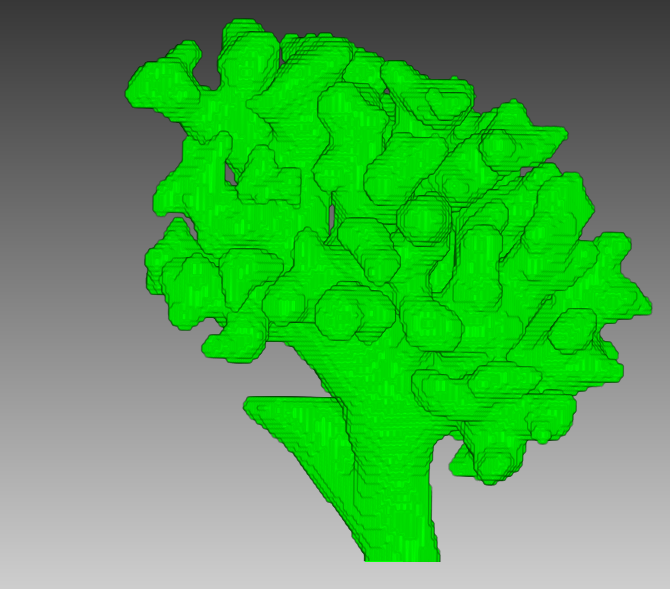
\includegraphics[width=\imagewidth]{img/skeleton/segment-crop0041}};
		\draw[|-|,thick] (25,550) -- (175,550) node[midway,above] {\unit{300}{\micro\meter}};
		\end{tikzpicture}}
		\subfloat[Overlay of \subref{fig:segment} and \subref{fig:skeleton}]{\label{fig:overlay}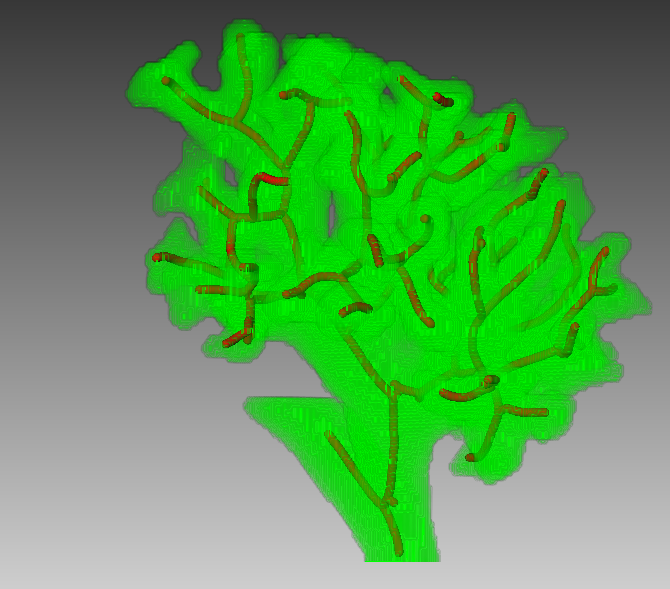
\includegraphics[width=\imsize]{img/skeleton/overlay-crop0041}}
		\subfloat[Skeleton]{\label{fig:skeleton}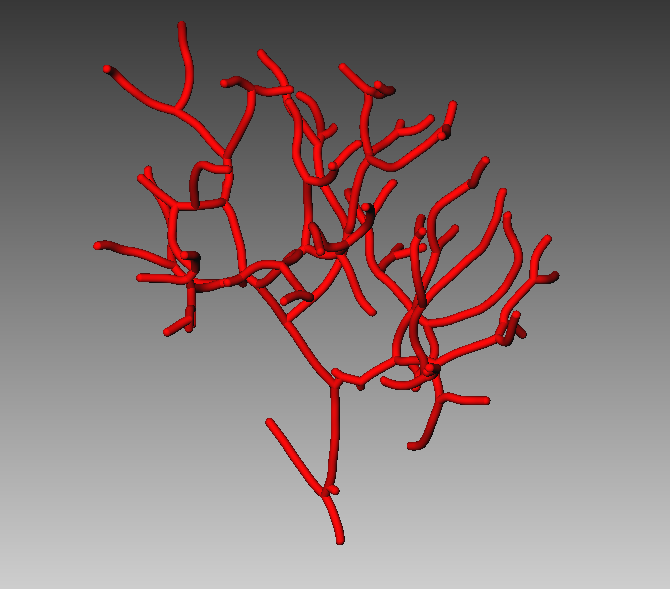
\includegraphics[width=\imsize]{img/skeleton/skel-crop0041}}
	\caption{Results of the skeletonization of the airways of a partial acinus from a Sprague Dawley rat four days after birth. An segmented acinus located at the tip of a scanned lung sample, directly underneath the pleura has been extracted from the tomographic dataset. A part of this segment has been used for the extraction of the skeleton, this part is shown in panel~\subref{fig:segment}. Panel \subref{fig:overlay} shows the skeleton inside the half transparent airway segment. The skeleton of the acinar airways is shown in red in panel~\subref{fig:skeleton}.}
	\label{fig:skeletonization}
\end{figure}

\section{Wide field scanning}
\label{sec:wide field scanning}
Various applications depend on the availability of high resolution tomographic images of the studied sample. The available field of view (FOV) of microscopy based imaging methods like SRXTM and \unit{\micro CT}{is} limited through the camera and microscope optics. The FOV can only be increased if the magnification of the microscope optics is decreased, thus decreasing the available resolution. At TOMCAT, the FOV varies from 11.4$\times$\unit{11.4}{\milli\meter} (1.25-fold magnification and 5.6$\times$\unit{5.6}{\micro\meter} pixel size) down to a FOV as low as 0.36$\times$\unit{0.36}{\milli\meter} for the highest resolution (40-fold magnification and 180$\times$\unit{180}{\nano\meter} pixel size).

The field of view can be enlarged by two different methods, by stacking multiple scans and by the so called wide field scanning, which has been developed and implemented at TOMCAT by me during the past year.

\subsection{Stacking of multiple Scans}
The FOV in the direction of the rotation axis of the sample can easily be enlarged by stacking multiple scans on top of each other. This is feasible for long and thin samples and has been implemented at TOMCAT through accurate control of the end-station setup and sample position and thorough calibration of the machine. A schematic drawing of this method is shown in figure~\ref{fig:stacking}.

\begin{figure}[tb]
	\centering
		%\documentclass{article}
%\usepackage[pdftex,active,tightpage]{preview}
%\usepackage{tikz}
%\usetikzlibrary{arrows,shapes,backgrounds}
%\begin{document}
%\begin{preview}
\begin{tikzpicture}[thick]%,show background grid]
	%draw axes
		%\draw[ultra thick] (-10,0) -- (10,0);
		%\draw[ultra thick] (0,-10) -- (0,10);
		%\draw[ultra thick] (0,0) circle (.125);
	% rotation axis
		\draw[->] (0,-2) ++ (-50:.75) arc (-50:300:.75 and .25);
		\draw (0,-3) node[below] {Rotation axis} -- ++(0,2);
		\draw[dotted] (0,-1) -- ++(0,2);
		\draw (0,1) -- ++(0,0.25);
		\draw[dotted] (0,1.25) -- ++(0,2);
	% position 1
		\draw (0,-1) circle (1.5 and .5);
		\fill[shade,semitransparent] (-1.5,-1) arc (-180:0:1.5 and .5) -- ++(0,2) arc (0:180:1.5 and .5) -- cycle;
		\draw (-1.5,-1) arc (-180:0:1.5 and .5) -- ++(0,2) arc (0:180:1.5 and .5) -- cycle;		
		\draw (-1.5,1) arc (-180:0:1.5 and .5);
		\draw (1.5,0) node[right] {First Position};
	% position 2
		\draw (0,1.25) circle (1.5 and .5);
		\fill[shade,semitransparent] (-1.5,1.25) arc (-180:0:1.5 and .5) -- ++(0,2) arc (0:180:1.5 and .5) -- cycle;
		\draw (-1.5,1.25) arc (-180:0:1.5 and .5) -- ++(0,2) arc (0:180:1.5 and .5) -- cycle;		
		\draw (-1.5,3.25) arc (-180:0:1.5 and .5);
		\draw (1.5,2.25) node[right] {Second Position};
	% rotation axis on top
		\draw[->] (0,3.25) -- ++(0,1.5);									
	% sample movement
		\draw[->] (-2.5,0) -- (-2.5,2) node [text width=1.75cm,midway,left] {Sample movement relative to beam and camera};	
\end{tikzpicture}
%\end{preview}
%\end{document}
	\caption{Increasing the field of view in vertical direction, feasible for long and thin samples. Two different scans are acquired and reconstructed. Thorough calibration ensures that the resulting image stacks can simply be stacked on top of each other. For illustration purposed the two positions are shown with a slight gap, in reality the sample is moved in such a fashion that the top slice of the data set obtained at the first position is adjacent to the bottom slice of the dataset obtained at the second position.}
	\label{fig:stacking}
\end{figure}

\subsection{Wide Field Scanning}
\label{sec:wfs-details}
Increasing the FOV in horizontal direction of the sample is not a similarly easy task, since the obtained projection images have to be merged together to one big projection prior to be able to reconstruct the tomographic dataset of the sample. A schematic drawing of such a wide field scan is shown in figure~\ref{fig:wide field scan setup}. Projection images of the central part of the sample are recorded, then the sample is moved laterally towards the side and projection images of the outer parts of the sample are obtained. All these projection images are subsequently stitched to projection images covering the full FOV.

To be able to reconstruct the virtual tomographic slices throughout the full sample diameter which is larger than the camera window, we need to obtain more projection images at the outer parts of the sample than at the inner parts of the sample. To fulfill the sampling theorem, we have to obtain $N$ projection images for a sample of the width of $N$ pixels for a \unit{180}{\degree} scan. If we e.\,g.\ have a camera which record 1024 pixels, we have to record at least 1024 projections over half a rotation. A consequence of this is, that we have to record more projections at the second position of the wide field scan, the outer ring. In this case, we have to record 1024$\times$3, therefore 3072 projections for half a rotation. If we record over one full rotations, i.\,e.\ a \unit{360}{\degree} scan, we record 6144 projections. We thus cannot simply merge together the projection images, but have to merge e.\,g.\ 6144 projections from the outer \unit{360}{\degree} scan with 1024 projections from the inner \unit{180}{\degree} scan to a total of 3072 merged projections for a \unit{180}{\degree} scan over three times the FOV of one standard scan.

\begin{figure}[tb]
	\centering
		%\documentclass{article}
%\usepackage[pdftex,active,tightpage]{preview}
%\usepackage{tikz}
%\begin{document}
%\begin{preview}
\begin{tikzpicture}[thick]%,show background grid]
	%draw axes
		%\draw[ultra thick] (-10,0) -- (10,0);
		%\draw[ultra thick] (0,-10) -- (0,10);
		%\draw[ultra thick] (0,0) circle (.125);
	% rotation axis
		\draw[->] (0,-3) ++ (-50:.75) arc (-50:300:.75 and .25);
		\draw[] (0,-4) node[below] {Rotation axis} -- ++(0,3);
		\draw[dotted] (0,-1) -- ++(0,2);
	% position 1
		\draw (0,-1) circle (1.5 and .5);
		\fill[shade,semitransparent] (-1.5,-1) arc (-180:0:1.5 and .5) -- ++(0,2) arc (0:180:1.5 and .5) -- cycle;
		\draw (-1.5,-1) arc (-180:0:1.5 and .5) -- ++(0,2) arc (0:180:1.5 and .5) -- cycle;		
		\draw (-1.5,1) arc (-180:0:1.5 and .5);
		\draw (1.25,-1.5) node[right] {First Position};
	% position 2
		\draw (0,-1) circle (4.5 and 1.5);
		\fill[shade,semitransparent] (-4.5,-1) arc (-180:0:4.5 and 1.5) -- ++(0,2) arc (0:180:4.5 and 1.5) -- cycle;
		\draw (-4.5,-1) arc (-180:0:4.5 and 1.5) -- ++(0,2) arc (0:180:4.5 and 1.5) -- cycle;		
		\draw (-4.5,1) arc (-180:0:4.5 and 1.5);
		\draw (2.25,-2.7) node[right] {Second Position};
	% top from position 1 on top
		\draw (0,1) circle (1.5 and .5);
	% rotation axis on top
		\draw[->] (0,1) -- ++(0,2.5);									
	% sample movement
		\draw[->] (0,1) -- (3,1) node [text width=3cm,above] {Sample movement relative to beam and camera};	
\end{tikzpicture}
%\end{preview}
%\end{document}
	\caption{Increasing the field of view in horizontal direction through so called wide field scanning. Details of the scanning method are described in section~\ref{sec:wfs-details}. Note that when one full scan has been performed, we can stack multiple wide field scans on top of each other as shown in figure~\ref{fig:stacking} to additionally increase the FOV in vertical direction.}
	\label{fig:wide field scan setup}
\end{figure}

The consequence of the sampling theorem implicates that the scanning time increases sevenfold for a threefold increase in lateral FOV (1024 projections for the inner, 6144 projections for the outer scan, in total 7168 projections) since the scanning time roughly scales with the total amount of obtained projections. During my master thesis I was able to show that the sampling theorem constraints mentioned above can be broken to a certain extent, while still allowing reconstructions of the sample without impairment in image quality.

I have written a MATLAB-script that asks the user for details about the sample and outputs different scanning protocols with varying amount of projections for the central and ring scans. The total amount of these projections scales with the scanning time and is plotted towards the expected reconstruction quality that can be expected. The results of a scan performed in such a way is shown in figure~\ref{fig:wide field scan results}. The parameters of this particular scan have been chosen in such a way that the total scanning time has been reduced by around \unit{60}{\%} compared to a standard scan while the reconstruction of the tomographic data still permits automatic segmentation of airway and tissue.

The wide field scanning method has been developed in close collaboration with the TOMCAT group not only for the needs of our group, but also for the implementation at the beamline for other users, so that tomographic reconstructions of samples with dimensions bigger than the camera window can be recorded. It has been implemented at the beamline for our needs, namely for the imaging of nearly full rat lung lobes where we want to extract the acinar airway skeleton as described in section~\ref{sec:skeletonization}. The full implementation at the beamline for all end-users is planned in spring 2009 after more tests and calibration scans have been carried out.

\begin{figure}
	\renewcommand{\imsize}{.16\linewidth}
	\pgfmathsetlength{\imagewidth}{\imsize} % desired display width of image
	\pgfmathsetlength{\imagescale}{\imagewidth/512} % pixel width of image
	\centering
		\subfloat[Three uncorrected projection images from the subscans s$_1$--s$_3$, each with a size of 1024$\times$1024 pixels at a resolution of \unit{1.4}{\micro\meter\per pixel}. 4676 projections have been acquired for the subscans s$_1$ and s$_3$, 1169 projections have been acquired for subscan s$_2$, all over a rotation of \unit{180}{\degree}.]{%
			\label{fig:s1}%
			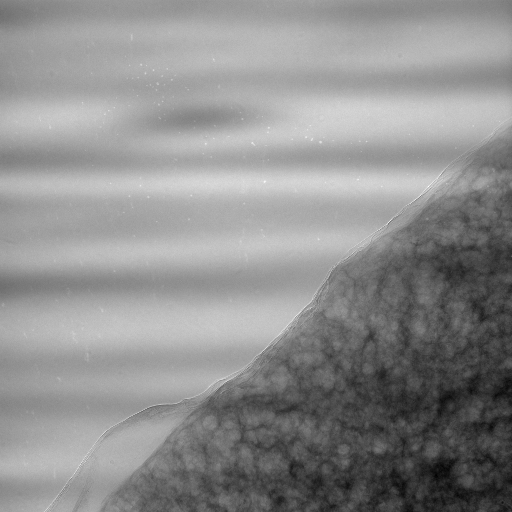
\includegraphics[width=\imsize]{img/merge/R108C10B-s1}%
			%}
			\
		%\subfloat[Uncorrected projection image from subscan s$_2$. 1169 projections like this one have been acquired over a rotation of \unit{180}{\degree}.]{%
		%	\label{fig:s2}%
			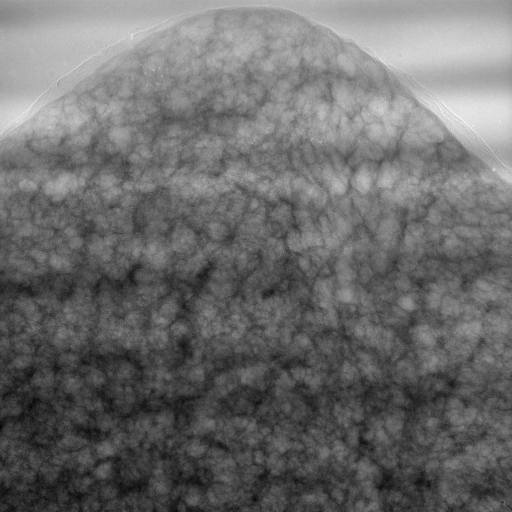
\includegraphics[width=\imsize]{img/merge/R108C10B-s2}%
		%	}
			\
		%\subfloat[Uncorrected projection image from subscan s$_3$. 4676 projections like this one have been acquired over a rotation of \unit{180}{\degree}.]{%
		%	\label{fig:s3}%
			\begin{tikzpicture}[x=\imagescale,y=-\imagescale]
				% place image (integer coordinates refer to pixel centers):
				\node[anchor=north west,inner sep=0pt,outer sep=0pt] at (0,0)
					{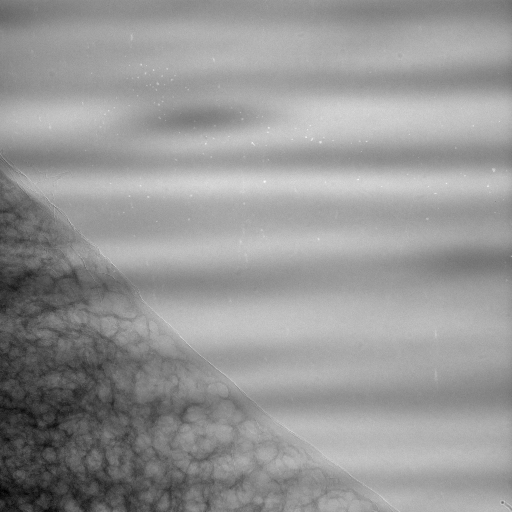
\includegraphics[width=\imagewidth]{img/merge/R108C10B-s3}};
				\draw[|-|,thick,color=white] (256-64,450) -- (512-64,450) node[midway,above] {\unit{700}{\micro\meter}};
				\end{tikzpicture}%
			\label{subfig:subscans}
			}
		\renewcommand{\imsize}{.47\linewidth}
		\pgfmathsetlength{\imagewidth}{\imsize} % desired displayed width of image
		\pgfmathsetlength{\imagescale}{\imagewidth/1498} % pixel width of image
		\subfloat[Merged and corrected image from the three subscans shown in subfigure~\subref{subfig:subscans}. The merged projections have a size of 2994$\times$1024 pixels at a resolution of \unit{1.4}{\micro\meter\per pixel}. The Subscans s$_1$--s$_3$ overlap each other by approximately 150 pixels, thus the width of the merged projection is smaller than three times the width of the subscans. The projections of the subscans above have been merged into 4676 projections images like the one shown here and were then reconstructed into a tomographic dataset using a filtered backprojection reconstruction algorithm.]{%
			\label{fig:merge-proj}%
			\begin{tikzpicture}[x=\imagescale,y=-\imagescale]
				% place image (integer coordinates refer to pixel centers):
				\node[anchor=north west,inner sep=0pt,outer sep=0pt] at (0,0)
					{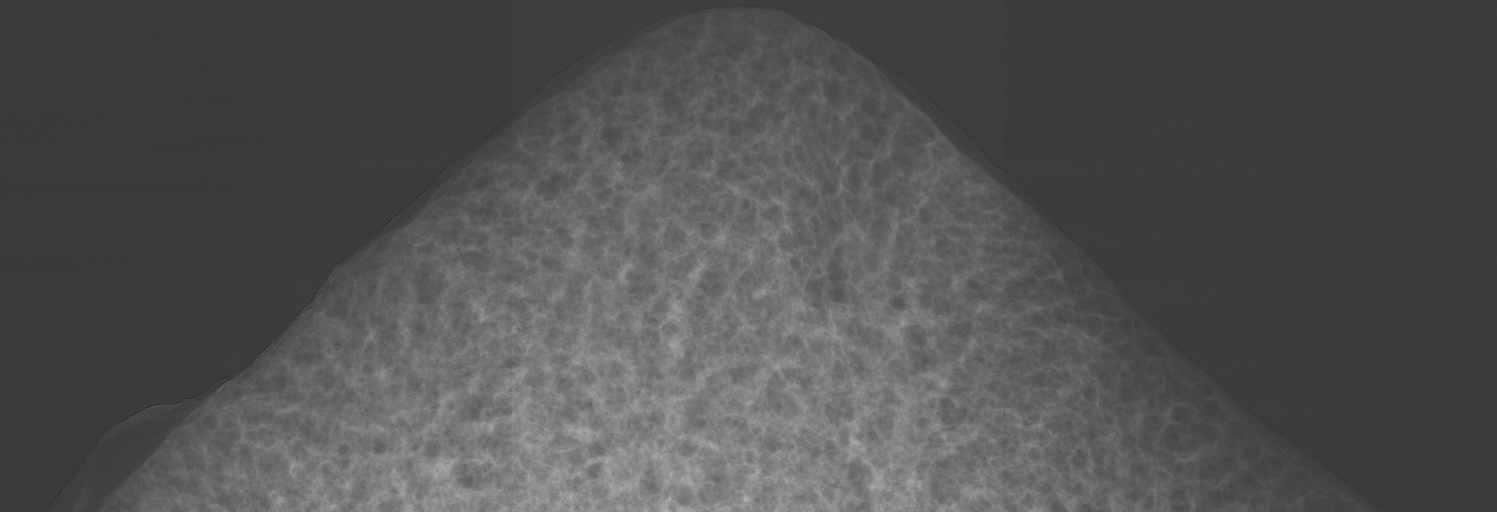
\includegraphics[width=\imagewidth]{img/merge/R108C10B-merge}};
				\draw[|-|,thick,color=white] (1242-64,450) -- (1498-64,450) node[midway,above] {\unit{700}{\micro\meter}};
			\end{tikzpicture}%
			}\\
		\renewcommand{\imsize}{\linewidth}
		\pgfmathsetlength{\imagewidth}{\imsize} % desired displayed width of image
		\pgfmathsetlength{\imagescale}{\imagewidth/1365} % pixel width of image (image has been resized from 2994*1123, so that scalebar is at the same height without calculating too much...)
		\subfloat[Cropped part of one slice of the tomographic dataset reconstructed from the merged projections, where one is shown in subfigure~\subref{fig:merge-proj}. The halo directly around the lung tissue arises from the paraffin where the sample is embedded in. The bright circular shape inscribed in the square arises from the filtered backprojection, the chosen reconstruction method. The size of the cropped image is 2994$\times$1123 pixels. The small inset on the upper left corner shows an overview over the full slice with a size of 2994$\times$2994 pixels.]{%
			\label{fig:merge-rec}%
			\begin{tikzpicture}[x=\imagescale,y=-\imagescale]
				% place image (integer coordinates refer to pixel centers):
				\node[anchor=north west,inner sep=0pt,outer sep=0pt] at (0,0)
					{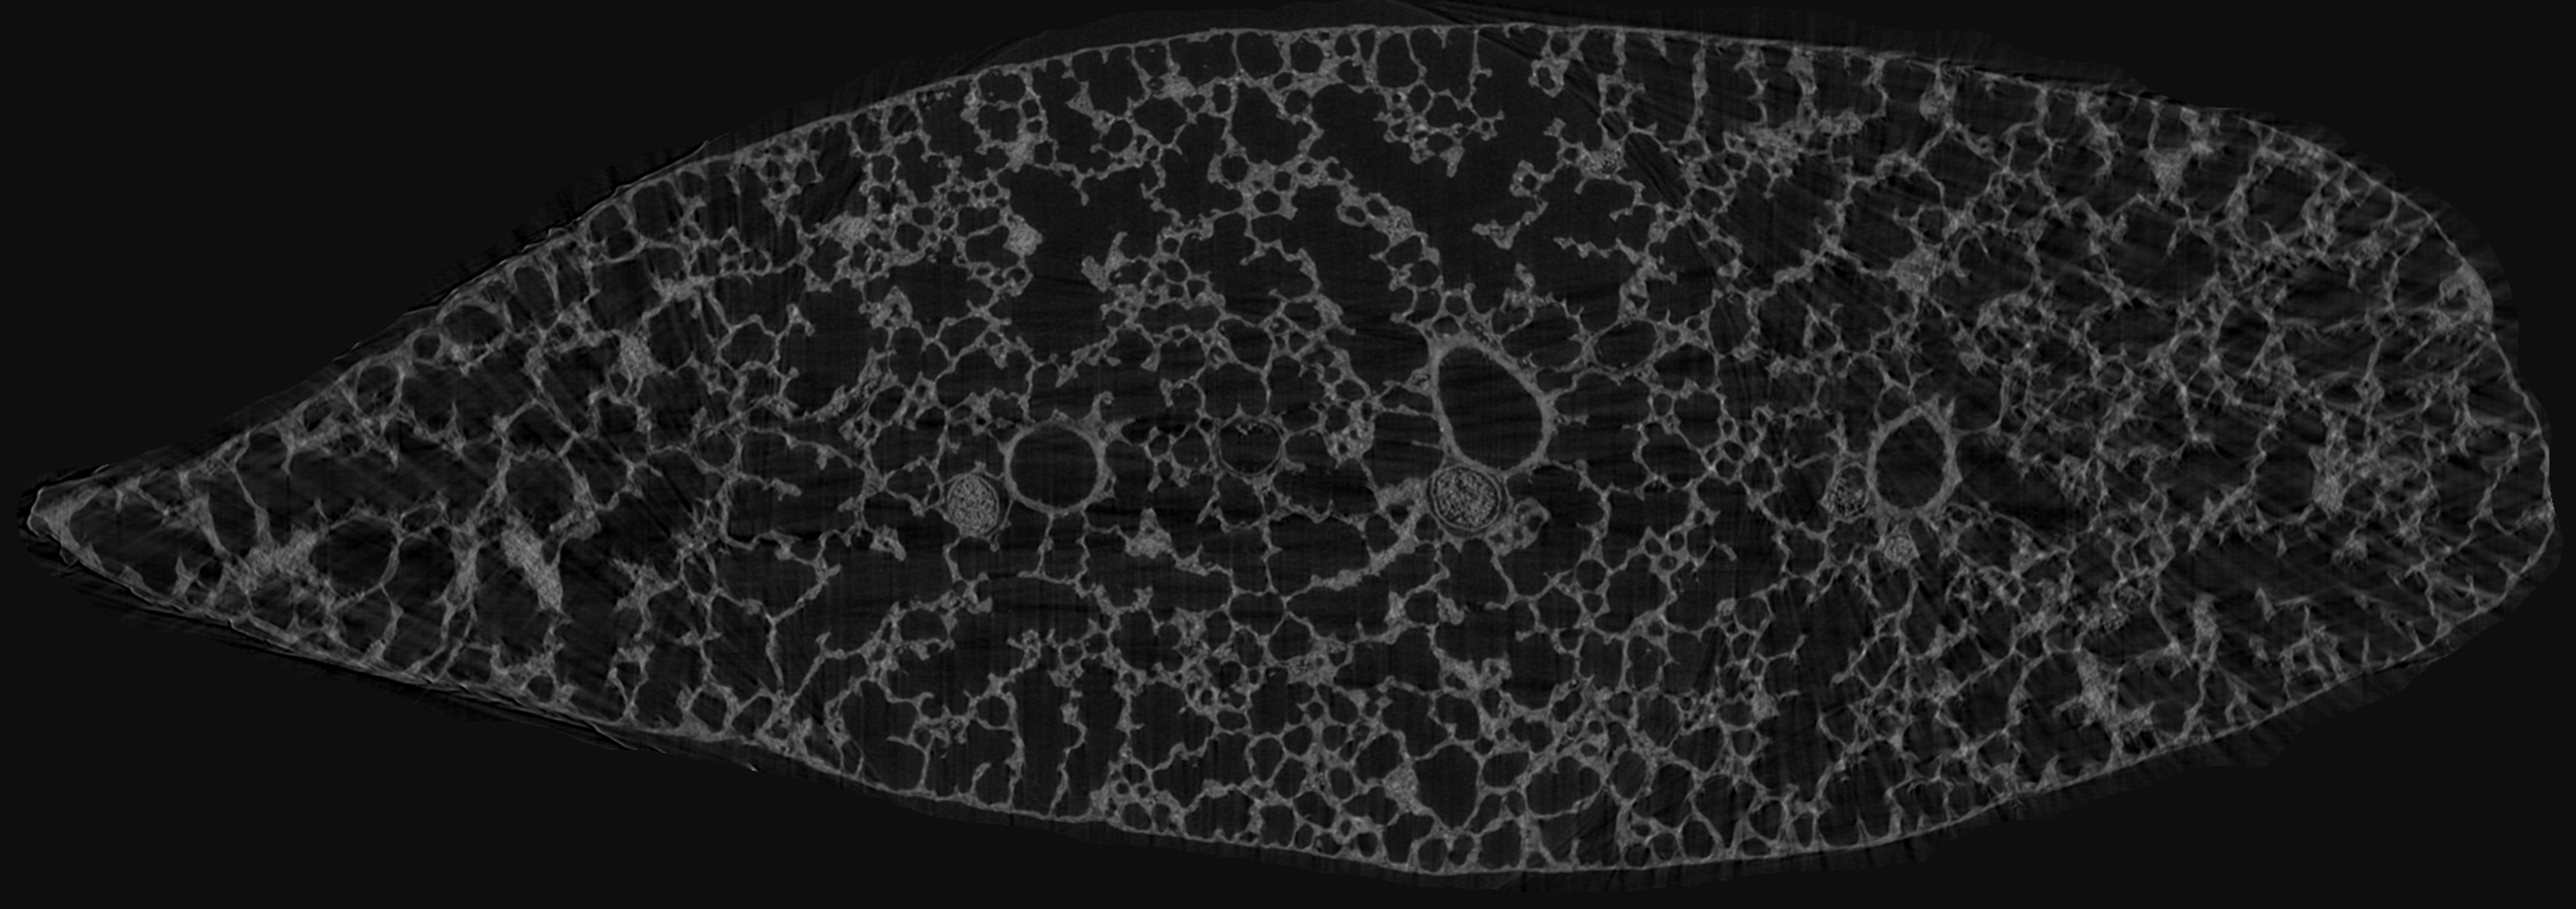
\includegraphics[width=\imagewidth]{img/merge/R108C10B-merge1016-crop}};
				\newcommand{\size}{.2\imagewidth}
				\node[anchor=north west,inner sep=0pt,outer sep=0pt] at (0,0)
					{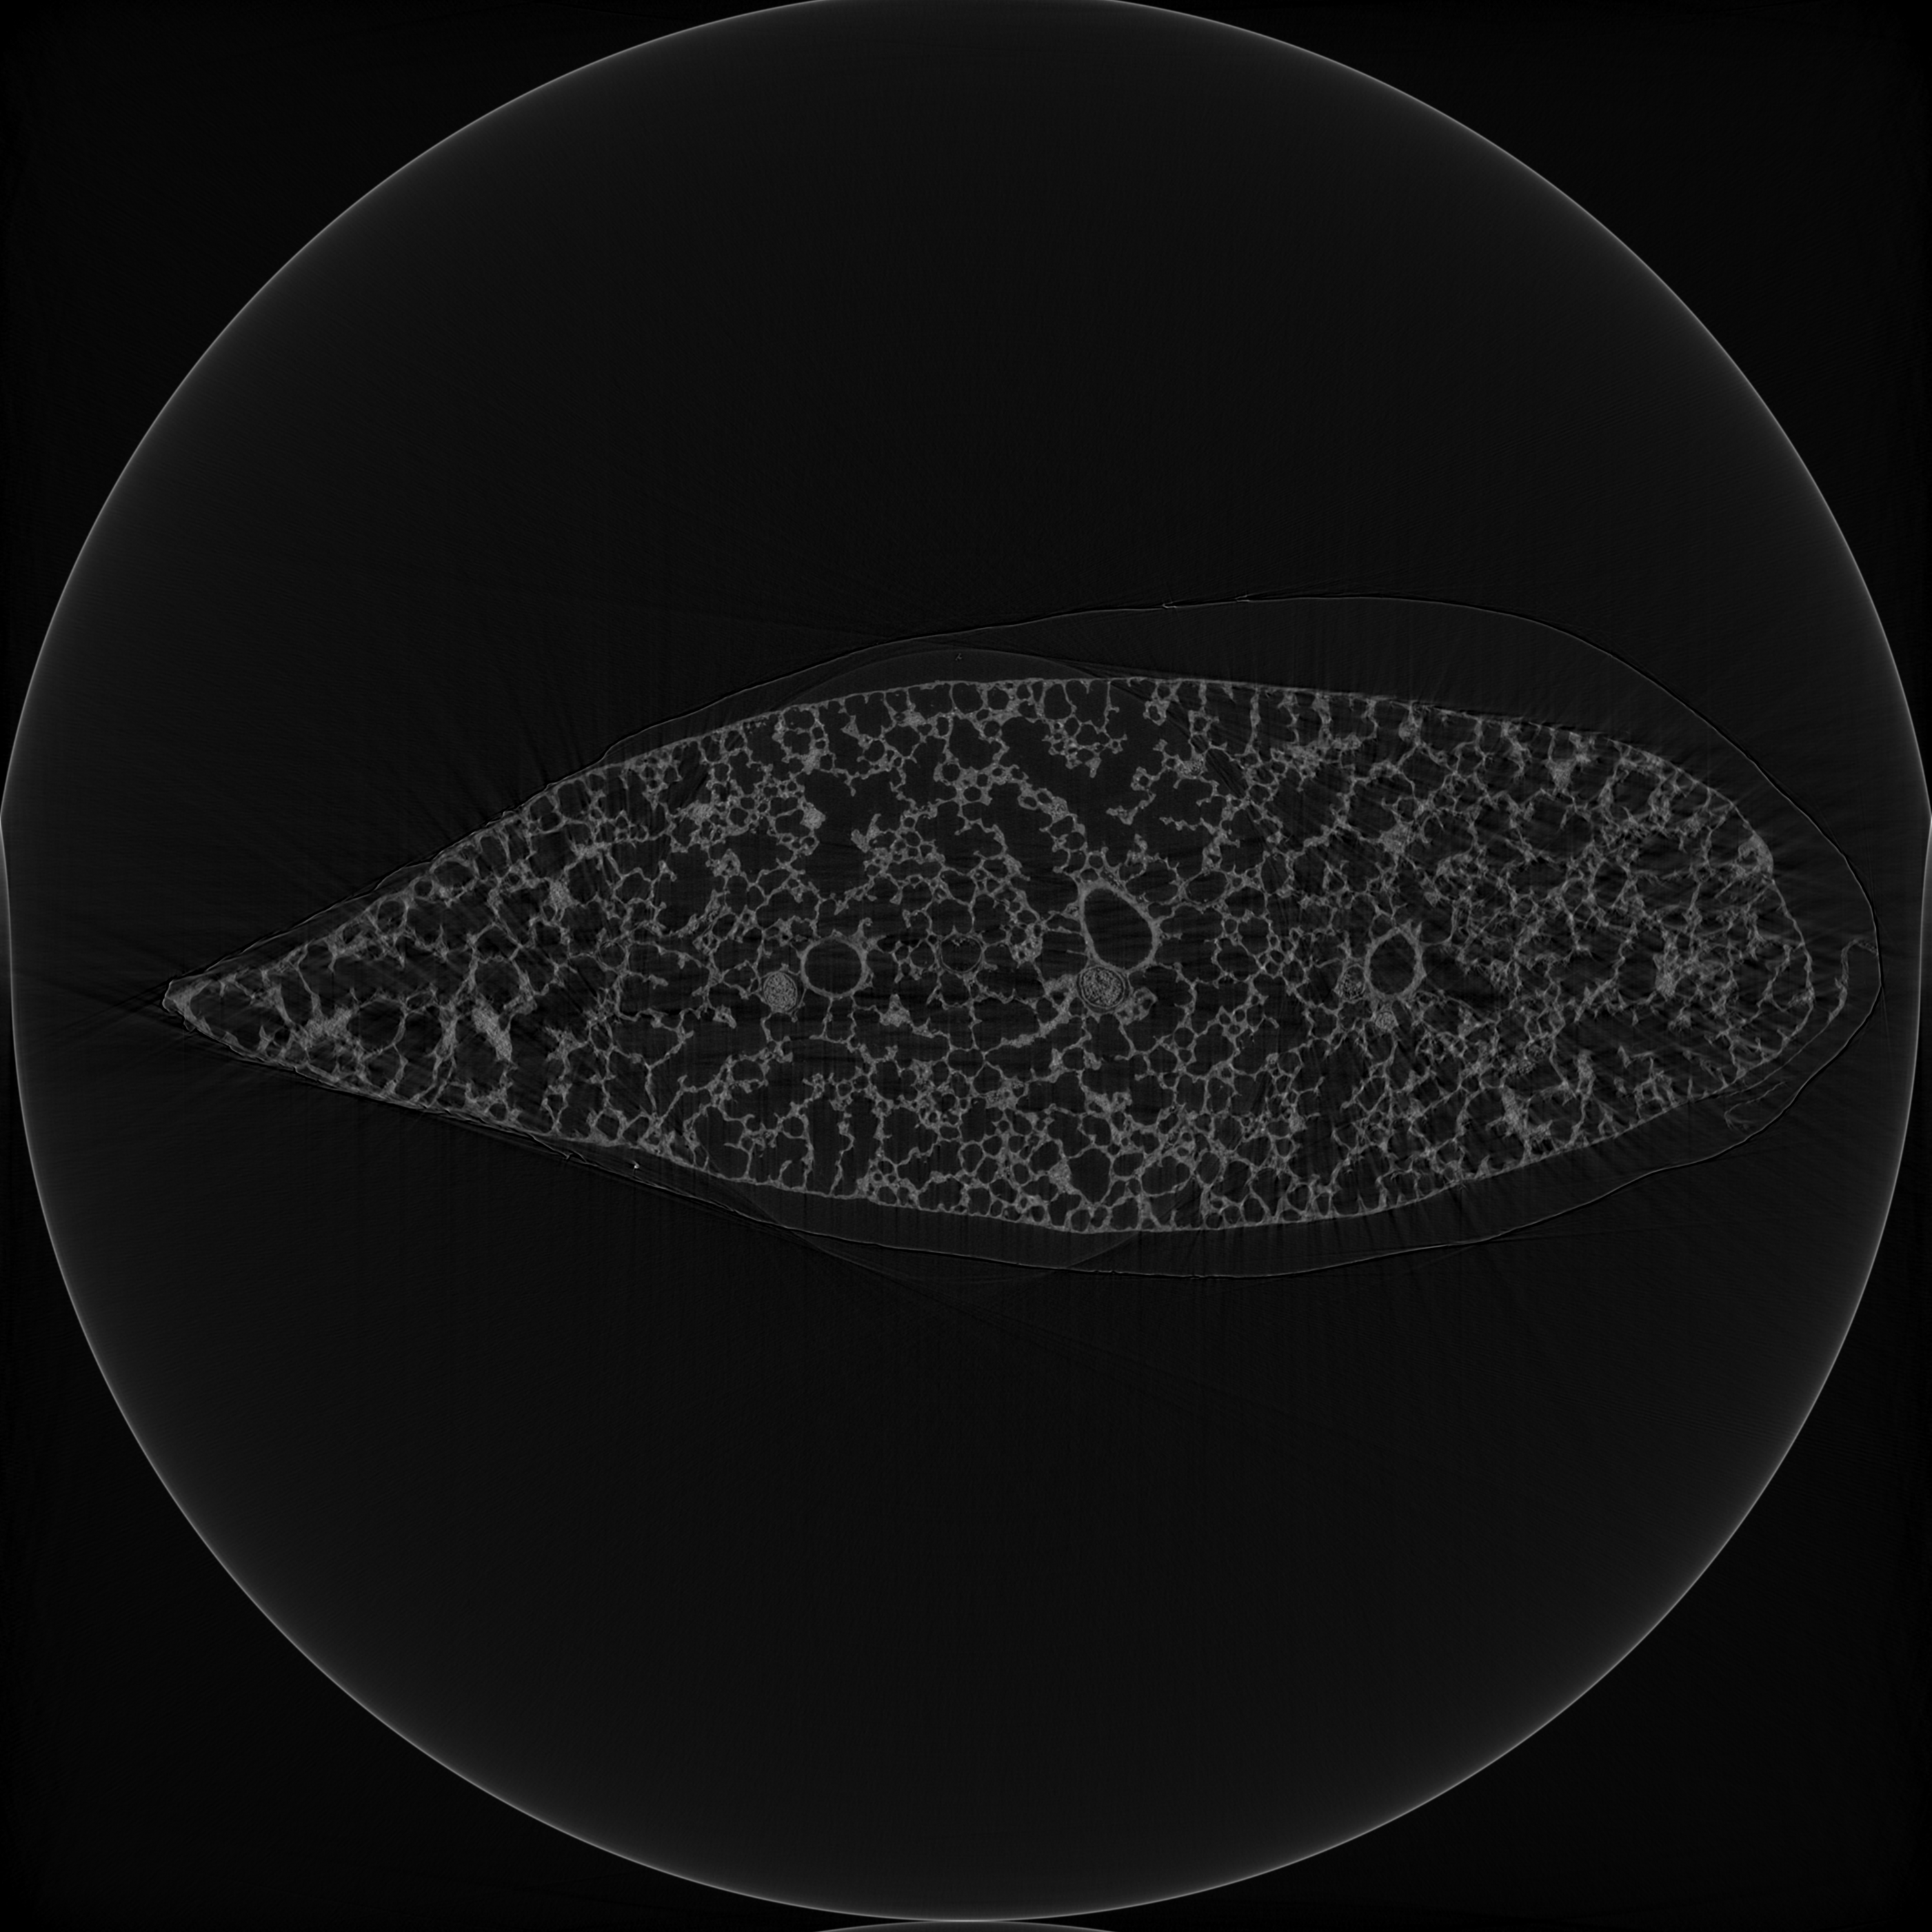
\includegraphics[width=\size]{img/merge/R108C10B-merge1016}};
					\draw[white] (\size,0) -- (\size,-\size) -- (0,-\size);
				\draw[|-|,thick,color=white] (1109-64,450) -- (1365-64,450) node[midway,above] {\unit{700}{\micro\meter}};
			\end{tikzpicture}%
			}\\
	\caption{Wide Field Scan Results for a rat lung sample 10 days after birth, showing the distal-medial edge of the right lower lung lobe.}
	\label{fig:wide field scan results}	
\end{figure}

\section{Publications}
\label{sec:publications}
Our group has been working on a publication to show the comparability of measurements obtained with SRXTM with classical morphological experiments. The paper~\cite{Tsuda2008} has been published this summer, I am one of the co-authors, have provided three figures and parts of the text.

As described in section~\ref{sec:multimodal imaging}, the multimodal imaging method has been successfully established at our institute. I have presented this method as a poster at two conferences~\cite{Haberthuer2008,Haberthuer2008b} and submitted a proceeding to the Journal of Physics~\cite{Haberthuer2009} after the second conference.

The preliminary results of my skeletonization method have been presented at a talk at the ``Tag der Anatomie''~\cite{Haberthuer2008a}, it is planned that---now that the method is applicable to our samples---we obtain more skeletons of terminal airways, study the arising alterations for different mouse strains and prepare a publication of this method.

The wide field scanning method has been thoroughly described in my master thesis of the MAS in Medical Physics~\cite{Haberthuer2008c} and presented to the other master students~\cite{Haberthuer2008d}. Currently, I am in the process of writing a publication now that additional experiments to prove the simulations and predictions have been carried out and showed the feasibility of the wide field scanning method.

\section{Outlook}
My experiments have shown that the wide field scanning method is ready to be implemented at the TOMCAT beamline. My MATLAB-scripts will be converted to faster routines programmed in \C++ by the beamline staff. There are still experiments needed to assess the long-term (in terms of hours) stability of the beamline setup and the reproducibility of the sample positioning. Preliminary results have been achieved by my, but the other assessments will be carried out by the beamline staff during in house development.

My skeletonization workflow still needs refinement. One of the main field I will work on in the next months is the extraction and visualization of different segments of the airway tree. Up to now we have a correct airway segment where we can manually detect the branching properties and generations of the tree. It would be desirable if we have an automatic mean of describing the mathematical properties of the tree like segment number, branching angles and Horsfield numbers~\cite{Horsfield1976}. This data is already present in the skeleton data which can be exported from MeVisLab as an XML-file. This file contains all the details like segment lengths, generations and branching angles. I am now working on the extraction and visualization of this data. This would then permit us to extract statistical information about the branching pattern of the acinar airway tree in different mice and rat strains and thus enable us to study differences in lung development on a quantitative level.

\bibliographystyle{unsrtnat}
\bibliography{../../references}

\end{document}